\documentclass[11pt]{article}
\usepackage{latexsym}
\usepackage{amsmath}
\usepackage{amssymb}
\usepackage{amsthm}
\usepackage{epsfig}
\usepackage[tight]{subfigure}
\usepackage{xcolor}
\usepackage{amsmath}
\usepackage{dsfont}
\usepackage{mathtools}
\usepackage{float}

\DeclareMathOperator*{\minimize}{min}
\DeclareMathOperator*{\maximize}{max}

\newcommand\defeq{\mathrel{\overset{\makebox[0pt]{\mbox{\normalfont\tiny\sffamily def}}}{=}}}


\usepackage{algorithm}
 %on linux you may need to run sudo apt-get install texlive-full to install algorithm.sys
\usepackage{algorithmic}

\usepackage{verbatim}

\usepackage[breaklinks=true,bookmarks=false]{hyperref}
\hypersetup{
    colorlinks=true,
    linkcolor=red,
    filecolor=magenta,      
    urlcolor=blue,
}

\newcommand{\handout}[5]{
  \noindent
  \begin{center}
  \framebox{
    \vbox{
      \hbox to 5.78in { {#1} \hfill #2 }
      \vspace{4mm}
      \hbox to 5.78in { {\Large \hfill #5  \hfill} }
      \vspace{2mm}
      \hbox to 5.78in { {\em #3 \hfill #4} }
    }
  }
  \end{center}
  \vspace*{4mm}
}

\newcommand{\lecture}[5]{\handout{#1}{#2}{#3}{#4}{#5}}
\newcommand{\collision}[0]{\mathrm{collision}}
\newcommand{\nocollision}[0]{\overline{\collision}}

\newcommand*{\QED}{\hfill\ensuremath{\square}}

\newtheorem{theorem}{Theorem}
\newtheorem{corollary}[theorem]{Corollary}
\newtheorem{lemma}[theorem]{Lemma}
\newtheorem{observation}[theorem]{Observation}
\newtheorem{proposition}[theorem]{Proposition}
\newtheorem{definition}[theorem]{Definition}
\newtheorem{claim}[theorem]{Claim}
\newtheorem{fact}[theorem]{Fact}
\newtheorem{assumption}[theorem]{Assumption}
\newtheorem{note}[theorem]{Note}

\newcommand{\indep}{\perp \!\!\! \perp}

% 1-inch margins, from fullpage.sty by H.Partl, Version 2, Dec. 15, 1988.
\topmargin 0pt
\advance \topmargin by -\headheight
\advance \topmargin by -\headsep
\textheight 8.9in
\oddsidemargin 0pt
\evensidemargin \oddsidemargin
\marginparwidth 0.5in
\textwidth 6.5in

\parindent 0in
\parskip 1.5ex
%\renewcommand{\baselinestretch}{1.25}
% \newtheorem{theorem}{Theorem}

\begin{document}

\lecture{Statistical Techniques in Robotics (16-831, S21)}{Lecture \#19
  (Wednesday, April 14)}{Lecturer: Kris Kitani}{Scribes: Akshay Dharmavaram, Zongyue Zhao}{Model-Free Value Prediction and Control}

\section{Review}

\subsection{Introduction}

In the previous lectures, we discussed various methods for on-policy model-free policy evaluation. Specifically, we covered the Monte Carlo (MC) method, one-step Temporal Difference (TD(0)), N-step TD, and the offline $\lambda$-Return method. We also proved that the TD error in $\lambda$-Return can be expressed as the weighted sum of a series of one step TD errors. In this lecture, we used this proposition to extend $\lambda$-Return to the online TD($\lambda)$, by introducing the concept of eligibility trace. Moreover, we discussed importance sampling and off-policy prediction, where the target policy - which is corresponding to the value function - is different from the sampling policy generating the trajectories.

In the following sections, we first provide a quick recap on the on-policy methods, which are characterized by the return estimate, then move on to the content of this lecture in details.

\subsection{Monte Carlo}

In general, the term "Monte Carlo" is used to describe a series of estimation methods that incorporate significant randomness \cite{sutton_reinforcement_1998}. In the context of reinforcement learning, MC methods refer to methods based on the average of complete sample returns. The return estimate for a single update is thus defined as:
\begin{equation}
    G^{(t)} = \sum_{i=t}^T r^(i)
\end{equation}

Here, because the sample return is not available until the episode is terminated, our algorithm is only incremental with respect to episodes, instead of actions. The benefit of doing so is that each estimate $G^{(t)}$ is a direct unbiased estimate of $V^{\pi}(s)$, and the average of these targets is still an unbiased estimator of the value function. On the other hand, the variance of such return-based target is high, especially when the sequence is long.

\subsection{Temporal Difference}

In order to address the shortcomings of MC methods, we introduced bootstrapping to incrementally update values after every action. Specifically, TD methods use a series of discounted rewards, which is a fragment of the total return, and the current estimate of the value function in place of the missing terms in the return, as the update target:
\begin{equation}
    G^{(t)}(N) = \sum_{i=t}^{t+N-1}\left(\gamma^{i-t}r^{(i)}\right)+\gamma^NV(s^{(t+N)})
\end{equation}
and the special case where $N=1$ is called TD(0):
\begin{equation}
    G^{t}_0\defeq G^{(t)}(1)= r^{t} + \gamma V(s^{(t+1)})
\end{equation}

Here, because we used the discounted value function in place of the missing terms in the true sampled return, each update is biased, and the more missing items (corresponding to a low $N$) the higher bias. However, these methods make it possible to update the value function incrementally with respect to actions, and thus the variance is lower.

\subsection{Offline $\lambda$-Return}

Finding the optimal $N$ in $TD(N)$ methods, i.e., finding the optimal point in the bias-variance trade-off, could be tricky. One method is to combine all temporal difference estimates by assigning higher weights to closer estimates, which is called $\lambda$-return:
\begin{equation}
    G_{\lambda}^{(t)} = (1-\lambda)\sum_{n=1}^\infty\lambda^{n-1}G^{(t)}(n)
    \label{lambda1}
\end{equation}
if the horizon of the task is infinite. For truly episodic tasks, the $\lambda$-return becomes:
\begin{equation}
    G_{\lambda}^{(t)} = (1-\lambda)\sum_{n=1}^{T-t-1}\left(\lambda^{n-1}G^{(t)}(n)\right) + \lambda^{T-t-1}G^{(t)}(T-t-1)
    \label{lambda2}
\end{equation}

Here, if the decay factor $\lambda$ is close to $0$, the algorithm heavily punishes estimates with long sample reward sequence, and the algorithm behaves like TD$(0)$. On the other hand, when the decay factor is close to $1$, the algorithm poses less punishment towards long estimates. In the extreme case where no decay is used ($\lambda=1$), the algorithm is simply Monte Carlo. 

Nonetheless, the $\lambda$-return method requires all TD updates up until the one extending to the end of the episode, thus the algorithm is offline (incremental w.r.t. episodes). In order to make $\lambda$-return an online algorithm, we need to express the corresponding TD error as a sum of weighted 1-step TD errors:
\begin{equation}
    \Delta V\left(s^{(t)}\right) = G_\lambda^{(t)} - V\left(s^{(t)}\right) = \sum_{i=0}^\infty (\gamma\lambda)^i\delta^{(t+i)}
    \label{Sum_weighted_1}
\end{equation}
where $\delta^{(\tau)}=r^{(\tau)}+\gamma V\left(s^{(\tau+1)}\right)-V\left(s^{(\tau)}\right)$ is the one-step TD error at $\tau$.

\section{Online TD ($\lambda$)}

\subsection{Eligibility Trace}

Consider the update rule of $\lambda$-return. If we use the offline target shown in Equation \ref{lambda1} or \ref{lambda2}, we are essentially looking forward in time to all future rewards, which are encoded in the various n-step TD errors, and try to find a way to optimally combine them. As shown in Figure \ref{fig:forward_view}, this is called the forward view of a learning algorithm. The problem of doing so is that it requires information of the unexplored parts of the trajectory when iterating through each time stamp, thus cannot be directly implemented online.

\begin{figure}
    \centering
    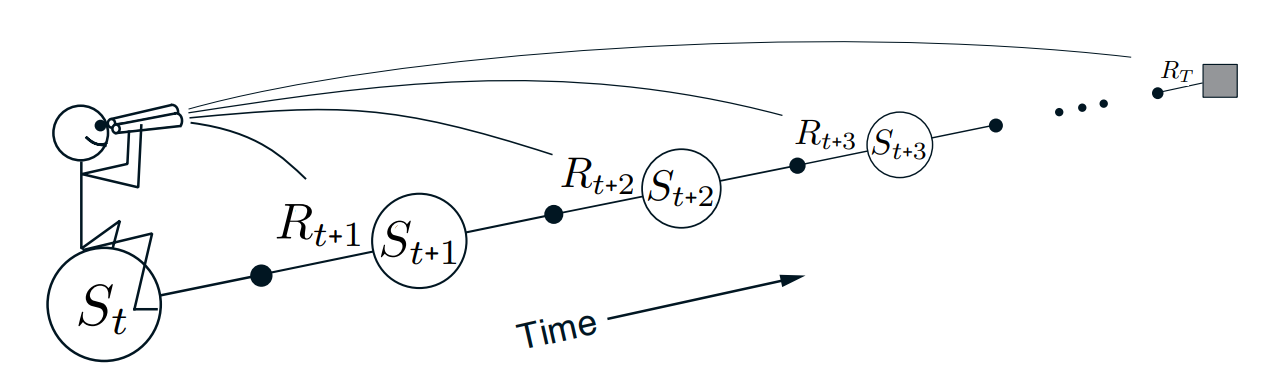
\includegraphics[width=0.8\textwidth]{forward.PNG}
    \caption{The Forward View \cite{sutton_reinforcement_1998}.}
    \label{fig:forward_view}
\end{figure}

One method of extending the offline $\lambda$-return algorithm is to introduce the concept of eligibility trace. Consider Equation \ref{Sum_weighted_1}, where we decomposed the TD error of the offline $\lambda$-return algorithm into the sum of a series of 1-step TD errors:
\begin{equation}
    \Delta V\left(s^{(t)}\right) = \sum_{i=0}^\infty (\gamma\lambda)^i\delta^{(t+i)}
    \label{eq:sum_2}
\end{equation}

Let us consider such an update on a specific state: suppose at timestamp $k$, $s^{(k)}=s$, then Equation \ref{eq:sum_2} can be written as:
\begin{equation}
    \Delta V\left(s^{(k)}=s\right) = \sum_{i=0}^\infty (\gamma\lambda)^i\delta^{(k+i)} = \sum_{t=k}^\infty (\gamma\lambda)^{t-k}\delta^{(t)}
\end{equation}
by shifting superscript notations.

The summation here begins from $t=k$, the current occurrence of $s$. For a consistent representation on the entire time horizon, we introduce zero-padding for time stamps prior to $t=k$, and the TD target now becomes:
\begin{equation}
    \Delta V\left(s^{(k)}=s\right) = \sum_{t=k}^\infty (\gamma\lambda)^{t-k}\delta^{(t)} = \sum_{t=1}^\infty z^{(t)}(s)\delta^{(t)}, \;\mathrm{where}\; z^{(t)}(s) = \bigg\{
    \begin{matrix*}[l]
    0 & t<k\\
    (\gamma\lambda)^{t-k}& t\geq k
    \end{matrix*}
\end{equation}

The weighting function $z^{(t)}(s)$ is called the eligibility trace. At this stage, we can use it to rewrite the $\lambda$-return update rule:
\begin{equation}
    V(s^{(t)}) \leftarrow V(s^{(t)}) + \alpha\Delta V\left(s^{(k)}=s\right)
\end{equation}
to:
\begin{equation}
    V(s) \leftarrow V(s) + \sum_{t=1}^\infty z^{(t)}(s)\delta^{(t)}
    \label{OFFLINE:ET}
\end{equation}

Note that the update rule \ref{OFFLINE:ET} is still offline when calculating explicitly, because it demands information from the entire horizon $t=1:\infty$. However, because of the structure of the eligibility trace $z^{(t)}$, we can adopt a recursive, online implementation by iterating through all states at each timestamp:
\begin{equation}
    \forall t, \forall s, z(s)\leftarrow \gamma\lambda z(s)+\mathds{1}[s^{(t)}=s]
\end{equation}

The reason we could not do so with the raw representation of $\Delta V\left(s^{(t)}\right) = G_\lambda^{(t)} - V\left(s^{(t)}\right)$ is that $G_\lambda^{(t)}$ spans in the entire episode horizon but $V\left(s^{(t)}\right)$ is a given value at the current timestamp, thus recursion is not available.

The full online algorithm is called $TD(\lambda)$, as shown in Algorithm \ref{TDLAMBDA}.

\begin{algorithm}[H]
\caption{TD($\lambda$-Prediction($\pi,\alpha,\lambda,\gamma,s^{(0)}$)}
\begin{algorithmic}
\label{TDLAMBDA}
\FOR{$s\in\mathcal{S}$}
\STATE $z(s)\leftarrow 0$ \hfill $\triangleright$ Initialize eligibility trace to zero vector.
\ENDFOR
\FOR{$t=0,...,T$}
\STATE $\{s^{(t+1)},a^{(t)},r^{(t)}\}\sim \mathcal{E}|\pi,s^{(t)}$ \hfill $\triangleright$ Select and execute action, receive reward
\STATE $\delta\leftarrow r^{(t)}+\gamma V\left(s^{(t+1)}\right)-V\left(s^{(t)}\right)$ \hfill$\triangleright$ 1-step TD error.
\FOR{$s\in\mathcal{S}$}
\STATE $z(s)\leftarrow \gamma\lambda z(s)+\mathds{1}\left[s^{(t)}=s\right]$ \hfill $\triangleright$ Update eligibility trace.
\STATE $V(s)\leftarrow V(s)+\alpha\delta z(s)$ \hfill $\triangleright$ Update value function
\ENDFOR
\ENDFOR
\RETURN $V(s)$
\end{algorithmic}
\end{algorithm}

Here, the online TD$(\lambda)$ algorithm adopts the backward view (note how the value function is updated for any state visited in the past, in a single timestamp, whereas in the forward view, only one - the current - state is updated in a single timestamp). Furthermore, an intuitive demonstration of TD$(\lambda)$ is shown in Figure \ref{fig:backward}: each update only depends on the current TD error combined with the eligibility traces summarizing past events.

\begin{figure}[ht]
    \centering
    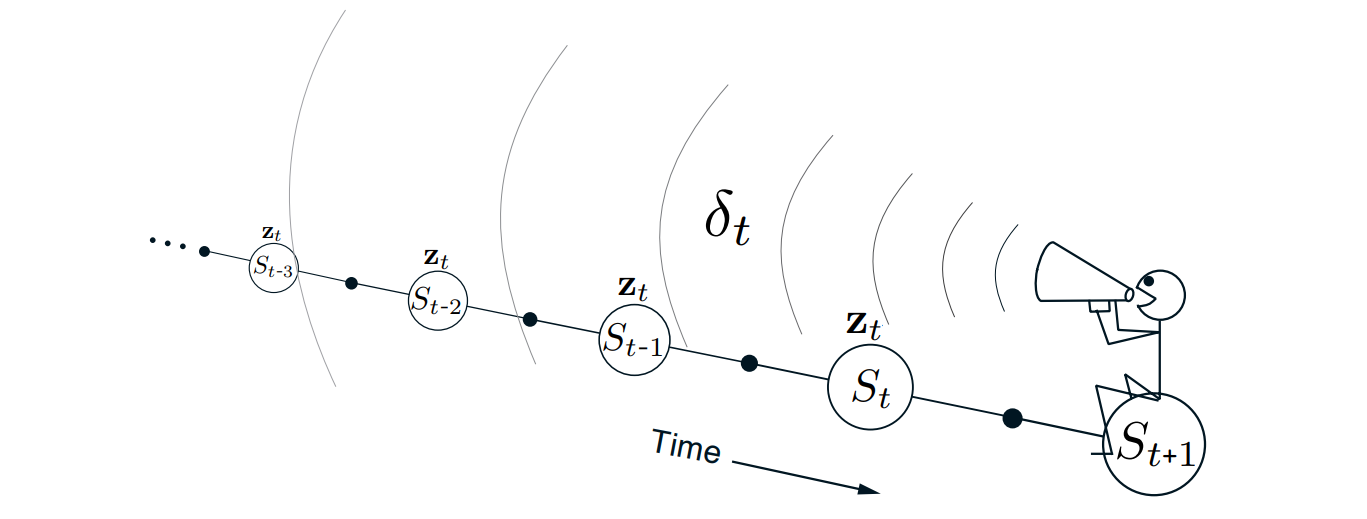
\includegraphics[width=0.8\textwidth]{backward.PNG}
    \caption{Backward View of TD$(\lambda)$ \cite{sutton_reinforcement_1998}}
    \label{fig:backward}
\end{figure}

The decay factor $\lambda$ controls the behavior of Algorithm \ref{TDLAMBDA}. When $\lambda=0$, which means $z(s)$ carries no information into the future, the algorithm simply yields the 1-step TD prediction (hence it is called $TD(0)$). On the other hand, when $\lambda=1$, there is no decay on the eligibility trace, and the algorithm becomes a variant of the discounted Monte Carlo Algorithm.

\section{Off-Policy Model-free Prediction}
\subsection{Off-Policy vs On-Policy}
Up until now, we have discussed the various on-policy model-free methods, and from here on we will be transitioning to off-policy methods. We will be discussing 2 methods, namely Importance Sampling for Off-policy MC Prediction (IS-MC) and Importance Sampling for Off-policy Temporal Differencing (IS-TD). 
\begin{table}[H]
\centering
\begin{tabular} { | p {2 cm} || p {3.7 cm} | p {4 cm} | }
\hline
Algorithms & Monte Carlo & Temporal Differencing \\
\hline
\hline
On-Policy & Monte Carlo & 1) N-step TD \\
&& 2) TD(lambda) \\
\hline
Off-Policy & Importance Sampling Monte-Carlo & Importance Sampling Temporal Differencing \\
\hline
\end{tabular}
\caption{Model-free Prediction Methods Covered}
\end{table}

Off-policy methods mainly defer from on-policy methods in their sampling steps. In an off-policy algorithm, we sample our state, action , and reward values from a distinct behavioral policy ($\mu$), which need not be our current target policy ($\pi$) that conditionally defines our value-function. Off-policy methods are useful in scenarios such as:
\begin{itemize}
    \item Learning a policy using the experience of other policies.
    \item Increasing the sample efficiency of traditional on-policy objectives.
    \item Evaluate multiple target policies using the experiences from a single behavioral policy.
    \item Evaluating a policy using different past experiences, defined by different behavioral policies.
\end{itemize}

As the samples in the off-policy setting are not from the target policy, if we keep the rest of the on-policy algorithm the same, we will end up converging upon the value-function that is conditioned over the behavioral policy ($\mu$) rather than the target policy ($\pi$). Thus, we will naturally have to change the value-function update equations to take into account the switch in the sampling procedure. We use the method of imporatnce sampling, to modify the value-function update steps, in order to obtain the correct value-function, which is conditioned on the target policy ($\pi$), instead of the behavioral policy ($\mu$).

In the upcoming sections, we will derive the the update equation involving importance sampling for the IS-MC and IS-TD methods, and finally, we will present the pseudocode for all the model-free prediction algorithms discussed till now.



\subsection{Importance Sampling for Off-policy MC Prediction}
In this section, we introduce the concept of importance sampling for off-policy MC prediction, and show how to update the value-function update steps, to converge upon the correct value-function. Importance sampling is a technique that helps us estimate the values of the value-function of the target policy, when given samples from a different a behavioral policy.

We will derive the importance sampling based update equation below. We start by expanding our value-function, based on our pre-defined definitions.

\begin{align} 
V^{\pi}(s) &=\mathbb{E}_{\pi}\left[G^{(t)} \mid s^{(t)}=s\right] \\ 
&=\sum_{s^{t+1: T}, a^{t: T-1}} \prod_{k=t}^{T-1} \pi\left(a^{(k)} \mid s^{(k)}\right) p\left(s^{(k+1)} \mid s^{(k)}, a^{(k)}\right) G^{(t)}
\end{align}

We can see that our current rollouts are conditional sampled from the target policy, $\pi$. Thus, we will introduce a trick that will help us transition the sampling process to one sampled by the behavioral policy, $\mu$. We multiply the numerator and the denominator with the corresponding sampled sequence from the behavioral policy, $\mu$. This does not affect the mathematical integrity of our update, as these values cancel out each other mathematically.

Next, we rearrange the numerator and the denominator to get a sampled sequence that is defined by our behavioral policy. 

\begin{align} 
V^{\pi}(s) 
&=\sum_{s^{t+1: T}, a^{t: T-1}} \frac{\prod_{k=t}^{T-1} \mu\left(a^{(k)} \mid s^{(k)}\right) p\left(s^{(k+1)} \mid s^{(k)}, a^{(k)}\right)}{\prod_{k=t}^{T-1} \mu\left(a^{(k)} \mid s^{(k)}\right) p\left(s^{(k+1)} \mid s^{(k)}, a^{(k)}\right)} \prod_{k=t}^{T-1} \pi\left(a^{(k)} \mid s^{(k)}\right) p\left(s^{(k+1)} \mid s^{(k)}, a^{(k)}\right) G^{(t)} \\
&=\sum_{s^{t+1: T}, a^{t: T-1}} \prod_{k=t}^{T-1} \mu\left(a^{(k)} \mid s^{(k)}\right) p\left(s^{(k+1)} \mid s^{(k)}, a^{(k)}\right) \frac{\prod_{k=t}^{T-1} \pi\left(a^{(k)} \mid s^{(k)}\right) p\left(s^{(k+1)} \mid s^{(k)}, a^{(k)}\right)}{\prod_{k=t}^{T-1} \mu\left(a^{(k)} \mid s^{(k)}\right) p\left(s^{(k+1)} \mid s^{(k)}, a^{(k)}\right)} G^{(t)} \\
&=\sum_{s^{t+1: T}, a^{t: T-1}} \prod_{k=t}^{T-1} \mu\left(a^{(k)} \mid s^{(k)}\right) p\left(s^{(k+1)} \mid s^{(k)}, a^{(k)}\right) \frac{\prod_{k=t}^{T-1} \pi\left(a^{(k)} \mid s^{(k)}\right)}{\prod_{k=t}^{T-1} \mu\left(a^{(k)} \mid s^{(k)}\right)} G^{(t)}
\end{align}

We finally reformulate the equation as an expectation and define a new importance sampling ratio $\frac{\prod_{k=t}^{T-1} \pi\left(a^{(k)} \mid s^{(k)}\right)}{\prod_{k=t}^{T-1} \mu\left(a^{(k)} \mid s^{(k)}\right)}$.

\begin{align} 
V^{\pi}(s) 
&=\mathbb{E}_{\mu}\left[\frac{\prod_{k=t}^{T-1} \pi\left(a^{(k)} \mid s^{(k)}\right)}{\prod_{k=t}^{T-1} \mu\left(a^{(k)} \mid s^{(k)}\right)} G^{(t)}\right] \\
&=\mathbb{E}_{\mu}\left[G_{\pi / \mu}^{(t)}\right]
\end{align}

The final value-function update can be summarized as 
\begin{align}
    \hat{V} (s_{t})=\hat{V} \left(s_{t}\right)+\alpha\left[G_{t}^{\pi / \mu}-\hat{V} (s_{t})\right]
\end{align}

\subsection{Importance Sampling for Off-policy Temporal Differencing}
In this section, we introduce the concept of importance sampling for off-policy TD prediction, and show how to update the value-function update steps, to converge upon the correct value-function. Importance sampling is a technique that helps us estimate the values of the value-function of the target policy, when given samples from a different a behavioral policy.

We will derive the importance sampling based update equation below. We start by expanding our value-function, based on our pre-defined definitions.

\begin{align}
V^{\pi}(s) &=\mathbb{E}_{\pi}\left[G^{(t)} \mid s^{(t)}=s\right]=\mathbb{E}_{\pi}\left[r^{(t)}+\gamma V^{\pi}\left(s^{(t+1)}\right) \mid s^{(t)}=s\right] \\
&=\sum_{s^{t+1}, a^{t}} \pi\left(a^{(t)} \mid s^{(t)}\right) p\left(s^{(t+1)} \mid s^{(t)}, a^{(t)}\right)\left(r^{(t)}+\gamma V^{\pi}\left(s^{(t+1)}\right)\right)
\end{align}
We can see that our current rollouts are conditional sampled from the target policy, $\pi$. Thus, we will introduce a trick that will help us transition the sampling process to one sampled by the behavioral policy, $\mu$. We multiply the numerator and the denominator with the corresponding sampled sequence from the behavioral policy, $\mu$. This does not affect the mathematical integrity of our update, as these values cancel out each other mathematically.

Next, we rearrange the numerator and the denominator to get a sampled sequence that is defined by our behavioral policy. 
\begin{align}
V^{\pi}(s) &=\sum_{s^{t+1}, a^{t}} \frac{\mu\left(a^{(t)} \mid s^{(t)}\right) p\left(s^{(t+1)} \mid s^{(t)}, a^{(t)}\right)}{\mu\left(a^{(t)} \mid s^{(t)}\right) p\left(s^{(t+1)} \mid s^{(t)}, a^{(t)}\right)} \pi\left(a^{(t)} \mid s^{(t)}\right) p\left(s^{(t+1)} \mid s^{(t)}, a^{(t)}\right)\left(r^{(t)}+\gamma V^{\pi}\left(s^{(t+1)}\right)\right) \\
&=\sum_{s^{t+1}, a^{t}} \mu\left(a^{(t)} \mid s^{(t)}\right) p\left(s^{(t+1)} \mid s^{(t)}, a^{(t)}\right) \frac{\pi\left(a^{(t)} \mid s^{(t)}\right)}{\mu\left(a^{(t)} \mid s^{(t)}\right)}\left(r^{(t)}+\gamma V^{\pi}\left(s^{(t+1)}\right)\right) 
\end{align}
We finally reformulate the equation as an expectation and define a new importance sampling ratio $\frac{\prod_{k=t}^{T-1} \pi\left(a^{(k)} \mid s^{(k)}\right)}{\prod_{k=t}^{T-1} \mu\left(a^{(k)} \mid s^{(k)}\right)}$.
\begin{align}
V^{\pi}(s) 
&=\mathbb{E}_{\mu}\left[ \underbrace{\frac{\pi\left(a^{(t)} \mid s^{(t)}\right)}{\mu\left(a^{(t)} \mid s^{(t)}\right)}}_\text{Importance weighting} \overbrace{\left(r^{(t)}+\gamma V^{\pi}\left(s^{(t+1)}\right)\right)}^\text{One-step TD estimate}\right]
\end{align}
The final value-function update can be summarized as 
\begin{align}
    \hat{V} (s_{t})=\hat{V} \left(s_{t}\right)+\alpha\left[\frac{\pi\left(a_{t} \mid s_{t}\right)}{\mu\left(a_{t} \mid s_{t}\right)}\left[r_{t}+\gamma \hat{V}\left(s_{t+1}\right)\right]-\hat{V} \left(s_{t}\right)\right]
\end{align}
\subsection{Off-policy vs On-Policy Temporal Differencing and MC Prediction}
In this section, we present the pseudo-code for the different model-free prediction algorithms presented thus far.

\begin{algorithm}[H]
\caption{MC-Prediction($\pi, \alpha$)}
\label{algo:MC}
\begin{algorithmic}[1]
\FOR{$e=1,\;\cdots,\;E$}
\STATE $\left\{s^{(t)}, a^{(t)}, r^{(t)}\right\}_{t=0}^{T} \sim \mathcal{E} \mid \pi$ \hfill $\triangleright$ Sampled from agent's current policy
\FOR{$t=0,\;\cdots,\;T$}
\STATE $G^{(t)} \leftarrow \sum_{i=t}^{T} r^{(t)}$  \hfill $\triangleright$ Summation of rewards
\STATE $V\left(s^{(t)}\right) \leftarrow V\left(s^{(t)}\right)+\alpha\left(G^{(t)}-V\left(s^{(t)}\right)\right)$ \hfill $\triangleright$ Value Function Update
\ENDFOR
\ENDFOR
\RETURN{} $V\left(s^{(t)}\right)$
\end{algorithmic}
\end{algorithm}

\begin{algorithm}[H]
\caption{TD-Prediction($\pi,\mu, \alpha, s^{(0)}$)}
\label{algo:TD}
\begin{algorithmic}[1]
\FOR{$t=0,\;\cdots,\;T$}
\STATE $\left\{s^{(t+1)}, a^{(t)}, r^{(t)}\right\} \sim \mathcal{E} \mid \pi, s^{(t)}$ \hfill $\triangleright$ Sampled from agent's current policy
\STATE $G^{(t)}(1)=\left(r^{(t)}+\gamma V^{\pi}\left(s^{(t+1)}\right)\right)$ \hfill $\triangleright$ Bootstrapped Value
\STATE $V^{\pi}\left(s^{(t)}\right) \leftarrow V^{\pi}\left(s^{(t)}\right)+\alpha\left(G^{(t)}(1)-V^{\pi}\left(s^{(t)}\right)\right)$ \hfill $\triangleright$ Value Function Update
\ENDFOR
\RETURN{} $V\left(s^{(t)}\right)$
\end{algorithmic}
\end{algorithm}
\begin{algorithm}[H]
\caption{OffPolicy-MC-Prediction ($\pi,\mu, \alpha$)}
\label{algo:MC1}
\begin{algorithmic}[1]
\FOR{$e=1,\;\cdots,\;E$}
\STATE $\left\{s^{(t)}, a^{(t)}, r^{(t)}\right\}_{t=0}^{T} \sim \mathcal{E} \mid \mu$ \hfill $\triangleright$ Sampled from behavioral policy
\FOR{$t=0,\;\cdots,\;T$}
\STATE $G^{(t)} \leftarrow \sum_{i=t}^{T} r^{(t)}$  \hfill $\triangleright$ Summation of rewards
\STATE $G_{\pi / \mu}^{(t)}=\frac{\prod_{k=t}^{T-1} \pi\left(a^{(k)} \mid s^{(k)}\right)}{\prod_{k=t}^{T-1} \mu\left(a^{(k)} \mid s^{(k)}\right)} G^{(t)}$ \hfill $\triangleright$ Importance sampling
\STATE $V^{\pi}\left(s^{(t)}\right) \leftarrow V^{\pi}\left(s^{(t)}\right)+\alpha\left(G_{\pi / \mu}^{(t)}-V^{\pi}\left(s^{(t)}\right)\right)$ \hfill $\triangleright$ Value Function Update
\ENDFOR
\ENDFOR
\RETURN{} $V\left(s^{(t)}\right)$
\end{algorithmic}
\end{algorithm}
\begin{algorithm}[H]
\caption{OffPolicy-TD-Prediction($\pi,\mu, \alpha, s^{(0)}$)}
\label{algo:TD1}
\begin{algorithmic}[1]
\FOR{$t=0,\;\cdots,\;T$}
\STATE $\left\{s^{(t+1)}, a^{(t)}, r^{(t)}\right\} \sim \mathcal{E} \mid \mu, s^{(t)}$ \hfill $\triangleright$ Sampled from behavioral policy
\STATE $G_{\pi / \mu}^{(t)}(1)=\frac{\pi\left(a^{(t)} \mid s^{(t)}\right)}{\mu\left(a^{(t)} \mid s^{(t)}\right)}\left(r^{(t)}+\gamma V^{\pi}\left(s^{(t+1)}\right)\right)$ \hfill  $\triangleright$ Importance sampling with bootstrapping
\STATE $V^{\pi}\left(s^{(t)}\right) \leftarrow V^{\pi}\left(s^{(t)}\right)+\alpha\left(G_{\pi / \mu}^{(t)}(1)-V^{\pi}\left(s^{(t)}\right)\right)$ \hfill $\triangleright$ Value Function Update
\ENDFOR
\RETURN{} $V\left(s^{(t)}\right)$
\end{algorithmic}
\end{algorithm}

\subsection{Review of Prediction Methods}
In this section, we will present a few tables summarizing the concepts presented over the past few lectures.

\begin{table}[H]
\centering
\begin{tabular} { | p {2 cm} || p {8 cm} | }
\hline
Algorithms & Return estimate $G^{(t)}$ \\
\hline
\hline
MC & $G^{(t)} =\sum_{i=t}^{T} r^{(i)} $ \\
TD(0) & $G_{0}^{(t)} =r^{(t)}+\gamma V\left(s^{(t+1)}\right)$ \\
N-step TD & $G^{(t)}(N) =\sum_{i=t}^{t+N-1} \gamma^{i-t} r^{(i)}+\gamma^{N} V\left(s^{(t+N)}\right)$ \\
$\lambda$-Return & $G_{\lambda}^{(t)} =(1-\lambda) \sum_{n=1}^{\infty} \lambda^{n-1} G^{(t)}(n)$ \\
TD($\lambda$) & $G_{z}^{(t)}  =z^{(t)}(s)\left[r^{(t)}+\gamma V\left(s^{(t+1)}\right)\right]$ \\
IS-MC & $G_{\pi / \mu}^{(t)} =\prod_{i=t}^{T} \frac{\pi\left(a^{(i)} \mid s^{(i)}\right)}{\mu\left(a^{(i)} \mid s^{(i)}\right)} \sum_{j=t}^{T} r^{(j)}$ \\
IS-TD(0) & $G_{\pi / \mu}^{(t)}(1)  =\frac{\pi\left(a^{(t)} \mid s^{(t)}\right)}{\mu\left(\left.a^{(t)}\right|_{s(t)}\right)}\left[r^{(t)}+\gamma V\left(s^{(t+1)}\right)\right]$ \\
\hline
\end{tabular}
\caption{Review of Prediction Methods}
\end{table}

\begin{table}[H]
\centering
\begin{tabular} { | p {2 cm} || p {9 cm} | }
\hline
Algorithms & Return estimate $G^{(t)}$ \\
\hline
\hline
MC & $G^{(t)} =\sum_{i=t}^{T} r^{(i)} $ \\
TD(0) & $G_{0}^{(t)}=r^{(t)}+\gamma Q\left(s^{(t+1)}, a^{(t+1)}\right)$ \\
N-step TD & $G^{(t)}(N)=\sum_{i=t}^{t+N-1} \gamma^{i-t} r^{(i)}+\gamma^{N} Q\left(s^{(t+N)}, a^{(t+N)}\right)$ \\
$\lambda$-Return & $G_{\lambda}^{(t)} =(1-\lambda) \sum_{n=1}^{\infty} \lambda^{n-1} G^{(t)}(n)$ \\
TD($\lambda$) & $G_{z}^{(t)}=z^{(t)}(s, a)\left[r^{(t)}+\gamma Q\left(s^{(t+1)}, a^{(t+1)}\right)\right]$ \\
IS-MC & $G_{\pi / \mu}^{(t)} =\prod_{i=t}^{T} \frac{\pi\left(a^{(i)} \mid s^{(i)}\right)}{\mu\left(a^{(i)} \mid s^{(i)}\right)} \sum_{j=t}^{T} r^{(j)}$ \\
IS-TD(0) & $G_{\pi / \mu}^{(t)}(1)=\frac{\pi\left(a^{(t)} \mid s^{(t)}\right)}{\mu\left(a^{(t)} \mid s^{(t)}\right)}\left[r^{(t)}+\gamma Q\left(s^{(t+1)}, a^{(t+1)}\right)\right]$ \\
\hline
\end{tabular}
\caption{Q-Value Equivalents}
\end{table}
\bibliography{refs}
\bibliographystyle{abbrv}


\end{document}



